\section{Introduction}

When Austrian born botanist Friedrich Reinitzer made the extraordinary observation in 1888 that a substance closely related to cholesterol had two melting points, one assumes he had no idea of the truly profound, awe-inspiring and beautiful branch of physics he was about to fore-father. His observation of a sample's transition from a solid crystal to a cloudy liquid at 145.5 $^{\circ}$C and from a cloudy liquid to a clear liquid at 178.5 $^{\circ}$C was without doubt, the first documented observation of the liquid crystalline phase of matter \citep{Reinitzer1888, Sluckin2004}.

In today's world, it's almost hard to believe that shortly after the second world war, scientific research in the field of liquid crystals slowed significantly due to the lack of a clear technological application. Conversely, at the time of writing, the majority of small to medium sized displays used \textit{worldwide} are liquid crystal devices. With more liquid crystal displays (LCDs) (be it pocket calculator or flat screen television) in existence than there are people living on planet earth \citep{Bruce2006}, it is of no surprise that the LCD industry was worth more than 60 billion US dollars in 2006, with projections estimating three fold increases in the coming years \citep{Bruce2006}. With the explosion of interest and research carried out in the field of liquid crystals from the 1970s to present (see Figure \ref{fig:web_of_science}), liquid crystal displays are now not only desired for their low cost, low power consumption and portability, but their attractiveness, ease of viewing and durability \citep{Collings1997}.

\begin{figure}
\begin{center}
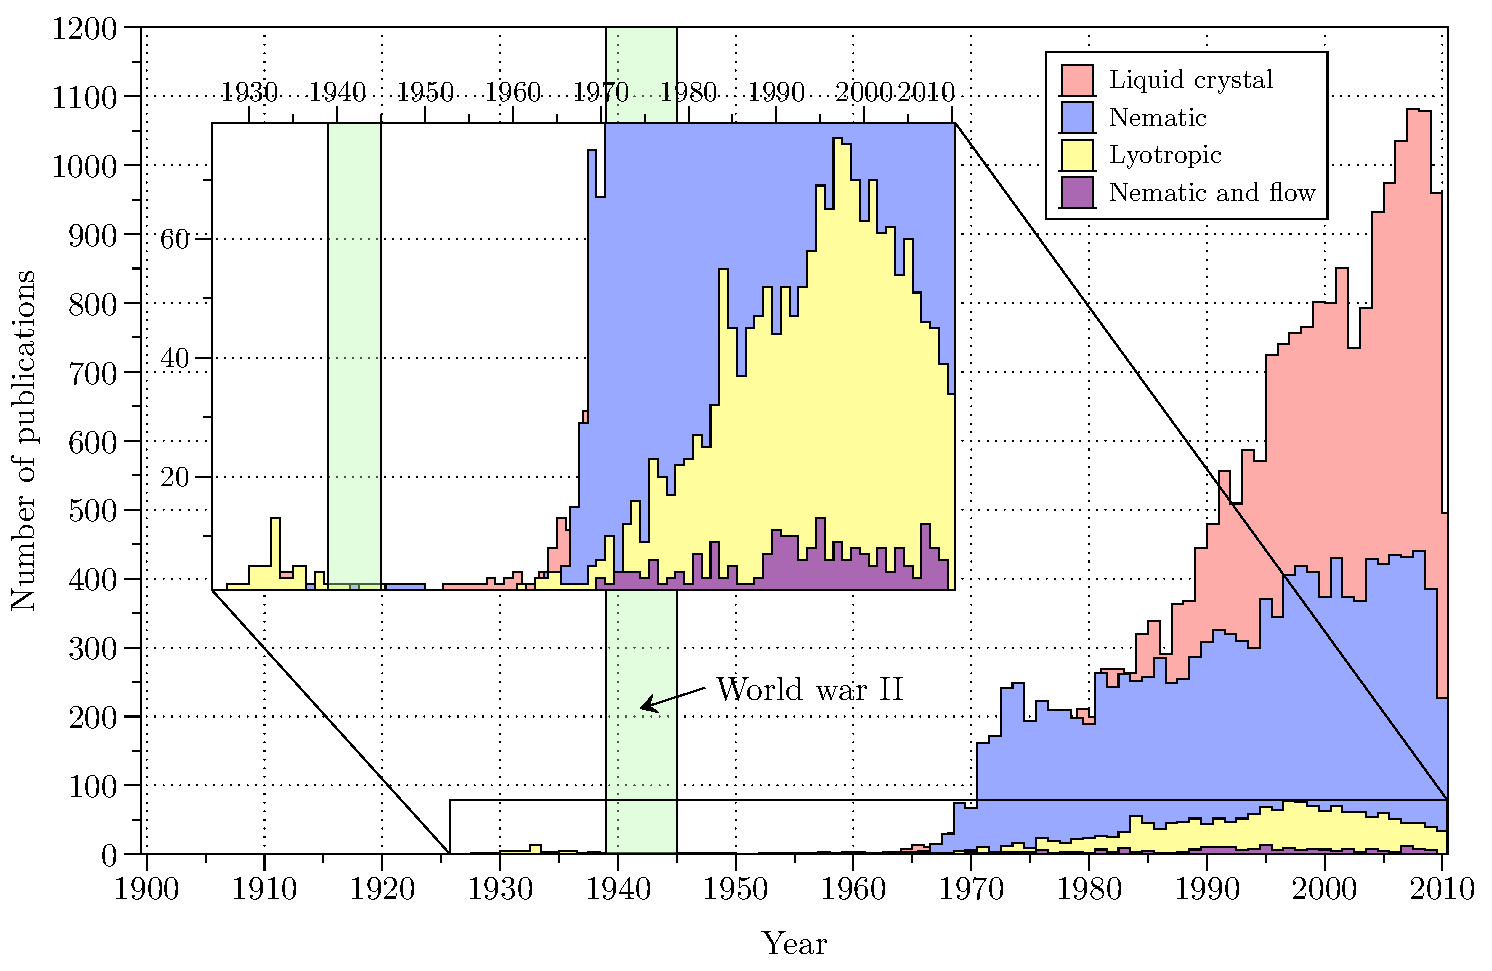
\includegraphics[width=0.48\textwidth]{figures/introduction/publications.pdf}
\caption[History of publications in the field of liquid crystal science (Source: Web of knowledge)]{\label{fig:web_of_science}A series of bar charts indicating the number of records on the Web of Science database that include in the article title the keyword shown in the legend. The lack of publications following World War II may be an artefact of the Web of Science database catalogue for these years. In any case, this figure serves to show the clear explosion in liquid crystal publication rates from 1970 onwards.}
\end{center}
\end{figure}

However, as is the case with any `state of the art' technology, it is destined to be quickly superseded by mankind's desire for faster, smaller, more efficient and simply better devices. With the new dawn in display screen technology arriving (OLEDs \citep{Burroughes1990}) we still find use for liquid crystal phases in other areas of science, as was highlighted recently at both the International Liquid Crystal Conference (ILCC 2010) in Krak\'{o}w and the European Conference on Liquid Crystals (ECLC 2011) in Slovenia.

Recent work such as that of Fleury \textit{et al.}\cite{Fleury2009} (the first winner of the Luckhurst Samulski prize \cite{Imrie2010}) is an excellent example of just how diverse and varied liquid crystal research can be. In their research, defect lines in nematic liquid crystal textures have been used to build metallic microwires, which allow for highly accurate electrode connections to be fabricated, down to the order of a few micrometers. This however, is just one example of recent pioneering work in the field of liquid crystal science. Many other examples of fascinating research in novel areas to liquid crystal scientists are being explored. These include but are not limited to, research into the dynamic diffusion of smectic layers \cite{Nguyen2010}, the production and  mechanical properties of spider's silk \cite{Vollrath2001,Lydon2004}, the use of liquid crystalline systems to model biological materials and processes \cite{Gupta2005} and the dynamics of fluid filaments, films, foams, bubbles and nematic shells \cite{Muller2007,Bird2010,Fernandez-Nieves2007}.
 
One particularly interesting area of research is involved with the striking similarity that certain liquid crystalline phases can share with specific organic viruses. Interest in this area has spanned the lifetime of liquid crystal research, originating with characterisation of the Tobacco Mosaic virus in 1936 \cite{Bawden1936}, through to cutting edge research on molecular permeation through smectic layers in a suspensions of `rod like' viruses \cite{Lettinga2007,Tkachenko1996, Helfrich1969}. There is also an entirely new branch of soft matter photonics being developed, based on nematic colloids \cite{Yablonovitch1987}, micro-lasers in liquid crystals \cite{Humar2010,Schafer2008,Doane1986} and optical trapping \cite{Smalyukh2005,Yada2004}.
 
That being said, there is still a wealth of interest and diversity within liquid crystal research, providing some of the most, in this author's opinion, interesting and often visually stimulating results. This introduction will now go on to give a brief outline of the content contained in the following chapters of this thesis.

\subsection{Thesis outline}
A general introduction to the liquid crystalline phase of matter is given in Chapter 2, titled \textit{`The liquid crystalline phase of matter'}.
 
Chapter 3, titled \textit{`Theory / Methods'} examines the underlying theory required to understand the workings and output of the one dimensional model of nematic liquid crystals dynamics that is used extensively throughout this thesis. This chapter also examines the experimental methods (namely optical conoscopy and flow cell fabrication) used in order to make measurements of nematic liquid crystals undergoing pressure driven flow.
 
In Chapter 4, titled \textit{`Flow alignment $\phi_0=45^{\circ}$}, a brief history of relevant flow experiments and processes is given before the results of a flow alignment experiment are presented, whereby optical conoscopy is used to measure the mean azimuthal rotation of the director when it is initially aligned at an azimuth of $45^{\circ}$ to the flow direction.

In Chapter 5, titled \textit{`Uniform and splayed pretilt profiles'}, the effect of surface pretilt on flow is experimentally investigated, with particular reference to the role of the two `uniform' and `splayed' alignment states that appear to lead to strikingly different director profiles when under flow. These experiments are conducted at an azimuthal angle close to normal to the flow direction.
 
Chapter 6, titled \textit{`Producing intermediate surface pretilt'} examines experimental techniques and recipes for producing much larger pretilt angles of the director at the cell walls (as can be commercially desirable), presenting interesting experimental data from two such recipes, here measured using a novel high-throughput technique.

Finally, Chapter 7 titled \textit{`Diode cell'} looks at the flow properties of a nematic liquid crystal exhibiting the large surface pretilt angles created using the research carried out in Chapter 6. Namely the idea of using a large pretilt angle in the `splayed' state as a valve, introducing the `diode' cell.
 
Chapter 8 then provides a summary and conclusion of the thesis, followed by a list of publications/presentations and bibliography.